\documentclass[]{article}

\usepackage[utf8]{inputenc}
\usepackage{amsmath}
\usepackage{multirow}
\usepackage{natbib}
\usepackage{graphicx} 
\usepackage{tabularx}



\begin{document}

\title{Mapping the Optimal Sensitivity of the 21 cm Forest to Dark Matter-Baryon Scattering}

\author{Denario}
\date{Anthropic, Gemini \& OpenAI servers. Planet Earth.}

\maketitle
\begin{abstract}
Elastic scattering between dark matter and baryons can suppress the formation of small-scale structure, offering a powerful observational test of dark matter microphysics. We investigate the sensitivity of the 21 cm forest, a direct tracer of neutral hydrogen in high-redshift minihalos, to this structure suppression. Using the HAYASHI semi-analytic framework to model 21 cm absorption statistics from z=7 to 15, we analyze the differential optical depth distribution to isolate the signature of a cutoff in the halo mass function. Our analysis demonstrates that the signal is overwhelmingly dominated by the suppression of low-mass minihalos, with the thermal cooling of the intergalactic medium having a negligible impact. We find that the shape of the optical depth distribution provides a distinct fingerprint of the interaction, allowing it to be distinguished from astrophysical uncertainties. Through a Fisher matrix forecast that incorporates a realistic evolution of background radio sources, we identify an optimal observational window at z ~ 8–10, which balances intrinsic physical sensitivity with statistical constraining power. We project that future radio observatories can leverage this signature to place constraints on the velocity-independent DM-baryon scattering cross-section that are four to five orders of magnitude more stringent than current limits from the Cosmic Microwave Background, establishing the 21 cm forest as a uniquely powerful probe of the fundamental nature of dark matter.
\end{abstract}








\section{Introduction}
\label{sec:intro}
The identity of dark matter constitutes one of the most significant unsolved problems in fundamental physics.\citep{bahcall2016dark} The standard cosmological paradigm, Lambda Cold Dark Matter ($\Lambda$CDM), provides an excellent description of the universe on large scales, from the anisotropies in the cosmic microwave background to the large-scale distribution of galaxies.\citep{van_den_Aarssen_2012,vandenaarssen2013is,chatterjee2024rulingstronglyinteractingdark,martins2009distributiondarkmattergalaxies,speliotopoulos2007darkenergystructureformation,teixeira2024illuminatingdarksectorsearching} However, the simple, non-interacting nature of cold dark matter is less rigorously tested on small scales, leaving a vast discovery space for new microphysical phenomena.\citep{van_den_Aarssen_2012,vandenaarssen2013is,chatterjee2024rulingstronglyinteractingdark,martins2009distributiondarkmattergalaxies,speliotopoulos2007darkenergystructureformation,brito2022snowmass2021cosmicfrontierwhite} Among the most compelling theoretical possibilities is the existence of a non-gravitational interaction between dark matter and baryons.\citep{van_den_Aarssen_2012,vandenaarssen2013is} If present, such an interaction would have left a distinct and potentially observable imprint on the formation of the very first cosmic structures.\citep{gluscevic2019cosmologicalprobesdarkmatter,chatterjee2024rulingstronglyinteractingdark,Wang_2016,brito2022snowmass2021cosmicfrontierwhite}

In the early universe, elastic scattering between dark matter and baryons would facilitate an exchange of momentum and heat, coupling the two fluids.\citep{tashiro2014effectsdarkmatterbaryonscattering,short2022darkmatterbaryonscatteringeffects} This coupling effectively acts as a pressure that counteracts gravitational collapse below a characteristic length scale, which is directly determined by the dark matter-baryon scattering cross-section. The primary cosmological consequence is a suppression of the matter power spectrum at high wavenumbers, which translates into a cutoff in the halo mass function.\citep{short2022darkmatterbaryonscatteringeffects,Sameie_2019,Schaeffer_2021,Bose_2019} This cutoff prevents the formation of the lowest-mass halos, thereby providing a direct link between the microphysics of dark matter and the abundance of small-scale structures.\citep{Sameie_2019,Diaz_Rivero_2018,moustakas2009stronggravitationallensingprobes,Schaeffer_2021} Searching for evidence of such a cutoff is therefore a powerful method for probing the fundamental properties of dark matter.\citep{Diaz_Rivero_2018,moustakas2009stronggravitationallensingprobes,Schaeffer_2021}

The 21 cm forest offers a uniquely direct window into this small-scale regime \citep{sun2025deeplearningdrivenlikelihoodfreeparameter,Shao_2023,Shao_2025,zhao202621cmforestonedimensional}. Arising from the absorption of radio waves from distant sources by intervening clouds of neutral hydrogen, the 21 cm forest traces the distribution of gas within the high-redshift intergalactic medium and inside the first gravitationally bound objects, known as minihalos \citep{sun2025deeplearningdrivenlikelihoodfreeparameter,Shao_2023,thyagarajan2020statisticaldetectionigmstructures,Xu_2009,Furlanetto_2002}. These minihalos are precisely the structures whose formation is most affected by a suppression of small-scale power \citep{sun2025deeplearningdrivenlikelihoodfreeparameter,Shao_2023,zhao202621cmforestonedimensional,Furlanetto_2002}. A key challenge, however, is that the statistics of 21 cm absorption lines are also sensitive to astrophysical effects, such as the intensity of the ambient ionizing background or the thermal state of the gas, creating potential degeneracies \citep{sun2025deeplearningdrivenlikelihoodfreeparameter,Shao_2023,šoltinský2025prospectsstatisticaldetection21cm,Shao_2025,Xu_2009}. The central problem is to develop an observational strategy that can robustly distinguish the signature of dark matter interactions from these astrophysical uncertainties \citep{sun2025deeplearningdrivenlikelihoodfreeparameter,Shao_2023,zhao202621cmforestonedimensional}.

In this paper, we quantify the optimal strategy for detecting the signature of dark matter-baryon scattering with the 21 cm forest . Using a semi-analytic framework to model the statistics of 21 cm absorbers, we demonstrate that the suppression of low-mass minihalos imprints a distinct feature on the shape of the optical depth distribution. This feature, a characteristic deficit of low optical depth systems, provides a powerful discriminant that allows the effects of dark matter microphysics to be disentangled from those of astrophysical parameters. We perform a Fisher forecast that incorporates a realistic, redshift-dependent evolution for the population of background radio sources to map the sensitivity of this probe across cosmic time \citep{Plombat_2025,Rahimieh_2025}. Our analysis identifies an optimal observational window at redshifts $z \sim 8-10$, where the combination of intrinsic physical sensitivity and statistical power is maximized. This work establishes a clear observational path for using next-generation radio observatories to place leading constraints on the nature of dark matter \citep{Rahimieh_2026,Murakami_2024,Plombat_2025,Rahimieh_2025}.

\section{Methods}
\label{sec:methods}
\subsection{Semi-analytic framework}

We model the statistics of the 21 cm forest using the \texttt{HAYASHI} semi-analytic framework \citep{Furlanetto_2002,Shao_2025,Xu_2009}. This code computes the distribution of neutral hydrogen absorbers along random lines of sight through the high-redshift universe, covering a redshift range from $z=7$ to $z=15$ \citep{Xu_2009,Furlanetto_2002,_oltinsk__2021,Shao_2025}. The model integrates contributions from both the diffuse intergalactic medium (IGM) and the dense gas residing within gravitationally bound minihalos, including both host halos and their subhalos \citep{Furlanetto_2002,_oltinsk__2021,Xu__2018}. For each line of sight, the framework calculates the 21 cm optical depth, $\tau$, which is inversely proportional to the gas spin temperature \citep{Xu_2009,šoltinský2025prospectsstatisticaldetection21cm}. This allows us to generate statistical distributions of absorption features, such as the cumulative number of absorbers above a certain optical depth, $N(>\tau)$, and the differential optical depth distribution, $dN/d\tau$ \citep{Furlanetto_2002,Shao_2025,šoltinský2025prospectsstatisticaldetection21cm}.

\subsection{Modeling dark matter-baryon scattering}

We incorporate the effects of elastic scattering between dark matter and baryons through two primary physical channels. The first and most significant channel is the suppression of small-scale structure \citep{Liu_2019,Dvorkin_2014,Slatyer_2018,tashiro2014effectsdarkmatterbaryonscattering,Rahimieh_2026,Halder_2021}. Momentum exchange between the two fluids damps primordial density fluctuations, leading to a cutoff in the matter power spectrum \citep{Dvorkin_2014,Liu_2019}. We model this effect by introducing a sharp cutoff in the halo mass function below a characteristic mass, $M_{cut}$ \citep{Liu_2019}. Halos with masses $M < M_{cut}$ are assumed not to form, directly reducing the population of low-mass minihalos that dominate the 21 cm forest signal \citep{Liu_2019,tashiro2014effectsdarkmatterbaryonscattering,Slatyer_2018,Halder_2021,Rahimieh_2026}.

The second channel is the thermal coupling between the two fluids. Heat transfer from the relatively warmer baryons to the colder dark matter can cool the IGM gas beyond the standard adiabatic expansion. \citep{Mu_oz_2017,short2022darkmatterbaryonscatteringeffects} We parameterize this effect with a cooling fraction, $f_{cool} = T_k / T_k^{ad}$, where $T_k$ is the kinetic temperature of the gas in the presence of scattering and $T_k^{ad}$ is the temperature from adiabatic cooling alone. Our analysis found the impact of this thermal channel on the 21 cm forest statistics to be negligible.

The cutoff mass $M_{cut}$ is directly related to the underlying dark matter-baryon scattering cross-section, $\sigma$ . We consider models where the cross-section has a power-law dependence on the relative velocity $v$, such that $\sigma = \sigma_0 v^n$ \citep{Mahdawi_2018,Rahimieh_2025}. Our analysis focuses on mapping constraints on $M_{cut}$ to the cross-section normalization $\sigma_0$ for two specific cases: a velocity-independent cross-section ($n=0$) and a Coulomb-like interaction ($n=-4$) \citep{Mahdawi_2018,Rahimieh_2025}.

\subsection{Statistical analysis and evaluation metrics}

Our analysis focuses on the differential optical depth distribution, $dN/d\tau$, as the primary observable. This distribution's shape is sensitive to the underlying population of absorbers \citep{filipp2026lsststronglensingsystems}. The suppression of low-mass halos due to dark matter-baryon scattering preferentially removes absorbers with low optical depth, imprinting a distinct "fingerprint" on the shape of the $dN/d\tau$ distribution .

To quantify the ability to distinguish a model with structure suppression from the standard $\Lambda$CDM scenario, we employ the Kullback-Leibler (KL) divergence \citep{Hee_2016,herrera2026informationtheoreticastrophysicaluncertaintieseffective}. The KL divergence, $D_{KL}(\text{CDM} \parallel M_{cut})$, measures the information gain when updating from a prior CDM distribution to a posterior distribution that includes a cutoff mass $M_{cut}$ \citep{Hee_2016,herrera2026informationtheoreticastrophysicaluncertaintieseffective}. A larger value of $D_{KL}$ indicates that the two distributions are more easily distinguishable, signifying greater intrinsic sensitivity to the effects of dark matter scattering \citep{herrera2026informationtheoreticastrophysicaluncertaintieseffective}.

\subsection{Fisher forecast methodology}

To project the observational capabilities of future radio observatories such as the Square Kilometre Array (SKA), we perform a Fisher matrix forecast \citep{Ewall_Wice_2016,Berti_2023,Balu_2023,Mason_2023}. The Fisher matrix, $F_{ij}$, quantifies the amount of information that an observable contains about a set of model parameters \citep{Mason_2023,Balu_2023,Ewall_Wice_2016,Alves_2017,sarkar2017fishermatrixbasedpredictions}. We construct the matrix for the parameter set $\{\theta_i\} = \{M_{cut}, f_{cool}, \bar{x}_{HI}\}$, where $\bar{x}_{HI}$ is the mean neutral hydrogen fraction \citep{Balu_2023,Mason_2023,Ewall_Wice_2016,zhang2025constrainingneutralhydrogenfraction}. The elements of the matrix are calculated as:
\begin{equation}
F_{ij} = \sum_{k} \frac{1}{N_k} \frac{\partial N_k}{\partial \theta_i} \frac{\partial N_k}{\partial \theta_j}
\end{equation}
where the sum is over bins of optical depth $\tau$, and $N_k$ is the number of absorbers in the $k$-th bin.\citep{Mallik_2024,2021}

A crucial element of our forecast is a realistic model for the number of available background radio sources, which we assume evolves with redshift \citep{Haiman_2004,massardi2010modelcosmologicalevolutionlow,Smol_i__2017,gao2024empiricalmodelextragalacticradio}. The number of lines of sight, $N_{los}$, is modeled as a power law:
\begin{equation}
N_{los}(z) = 10 \left( \frac{1+z}{8} \right)^{-2.5}
\end{equation}
This accounts for the increasing scarcity of bright radio-loud quasars at higher redshifts. The statistical uncertainty on the number of absorbers in each bin is assumed to be Poissonian, scaling with $1/\sqrt{N_{los}}$. By inverting the Fisher matrix, we obtain the covariance matrix, from which we extract the marginalized 1-$\sigma$ uncertainty on our parameter of interest, $\sigma(M_{cut})$ \citep{Porter_2015}. This forecast allows us to identify the optimal observational redshift window that balances intrinsic physical sensitivity with statistical constraining power \citep{wolfson2023forecastingconstraintshighzigm}.

\section{Results}
\label{sec:results}
Our analysis reveals that the 21 cm forest is an exceptionally sensitive probe of dark matter-baryon scattering, an effect driven almost entirely by the suppression of small-scale structure. We first disentangle the impacts of structure suppression and thermal cooling, then quantify the unique signature imprinted on the optical depth distribution, and finally forecast the observational constraints on the scattering cross-section.

\subsection{Dominance of structure suppression over thermal effects}

Dark matter-baryon scattering impacts the 21 cm forest through two primary physical channels: the kinematic suppression of low-mass halos and the thermal cooling of the intergalactic medium (IGM). Our analysis reveals a stark dichotomy in their observational significance, with structure suppression being the overwhelmingly dominant effect.

The thermal channel, parameterized by the cooling fraction $f_{\text{cool}} = T_k / T_k^{\text{ad}}$, has a negligible impact on the 21 cm forest statistics. As shown in the middle panel of Figure \ref{fig:image0}, even extreme cooling ($f_{\text{cool}} \to 0.02$) produces no discernible change in the cumulative number of absorbers, $N(>\tau)$. This is because the 21 cm optical depth is inversely proportional to the spin temperature, which is already very low in the cold, high-redshift IGM. The absorption signal is effectively saturated, and further cooling induced by scattering does not significantly alter the absorption profile. Across all redshifts studied, the maximum fractional change in the total number of absorbers due to cooling remains below $0.002\%$.

In stark contrast, the suppression of small-scale structure, parameterized by the cutoff mass $M_{\text{cut}}$, has a profound effect. The left panel of Figure \ref{fig:image0} shows that increasing $M_{\text{cut}}$ leads to a dramatic reduction in the number of absorbers at all optical depths. This occurs because the interaction damps primordial density fluctuations, preventing the formation of the low-mass minihalos that are the primary hosts of 21 cm absorbers. This powerful effect is further illustrated in Figure \ref{fig:image2}, which quantifies the fractional change in the total absorber count across redshift. A modest cutoff of $M_{\text{cut}} = 10^4 \, M_\odot$ reduces the absorber count by $50.2\%$ at $z=7$ and $47.0\%$ at $z=10$. For stronger interactions corresponding to $M_{\text{cut}} \ge 10^6 \, M_\odot$, over 92\% of the absorbers are eliminated. This establishes that the kinematic suppression of minihalo formation is the overwhelmingly dominant signature of dark matter-baryon scattering in the 21 cm forest.

\begin{figure*}[t]
    \centering
    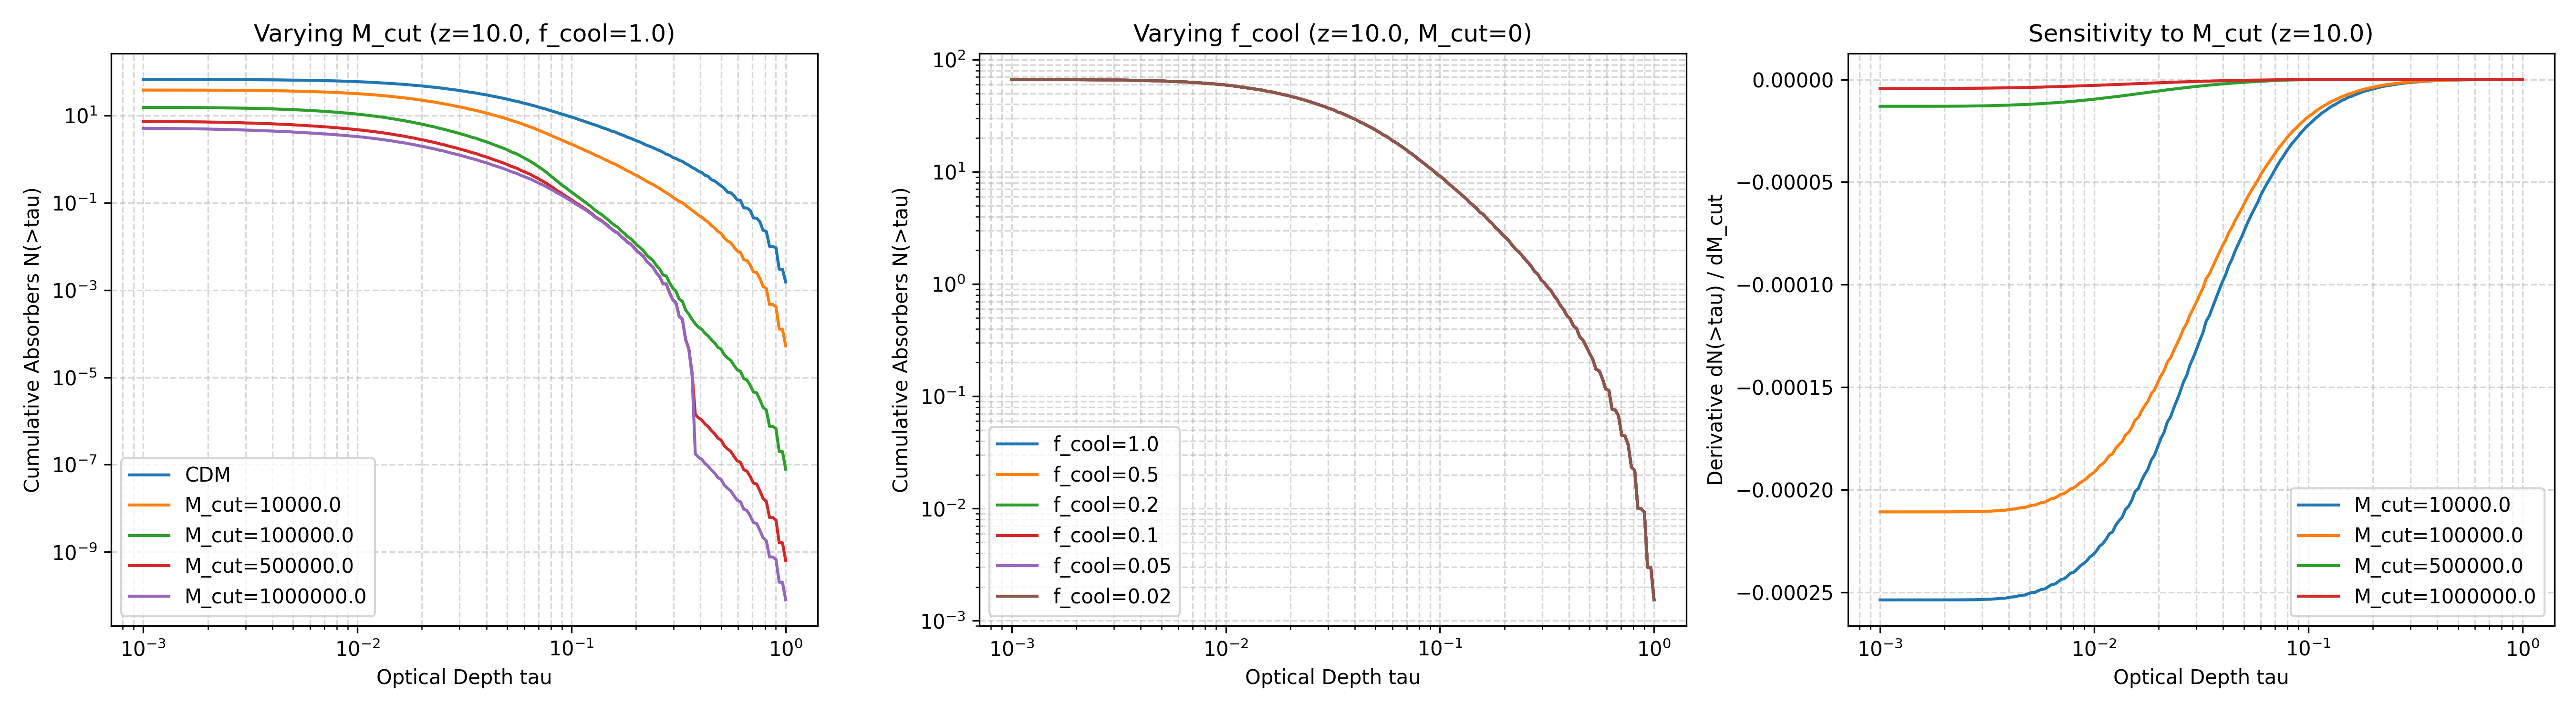
\includegraphics[width=\textwidth]{../input_files/plots/step_2_N_tau_and_derivative_1_20260413_122322.png}
    \caption{The differential impact of structure suppression versus thermal cooling on the 21 cm forest at redshift $z=10$. The cumulative number of absorbers above an optical depth $\tau$, $N(>\tau)$, is strongly suppressed with increasing halo mass cutoff, $M_{\text{cut}}$ (left panel), as dark matter-baryon scattering eradicates the low-mass minihalos that dominate the absorber population. In contrast, the thermal cooling channel, parameterized by the cooling fraction $f_{\text{cool}}$, has a negligible effect on the absorber count (middle panel) due to signal saturation in the cold intergalactic medium. The derivative of the cumulative distribution with respect to the cutoff mass, $\partial N(>\tau) / \partial M_{\text{cut}}$ (right panel), reveals that the suppression is most pronounced at low optical depths, providing a distinct spectral fingerprint for this interaction.}
    \label{fig:image0}
\end{figure*}

\begin{figure}[h!]
    \centering
    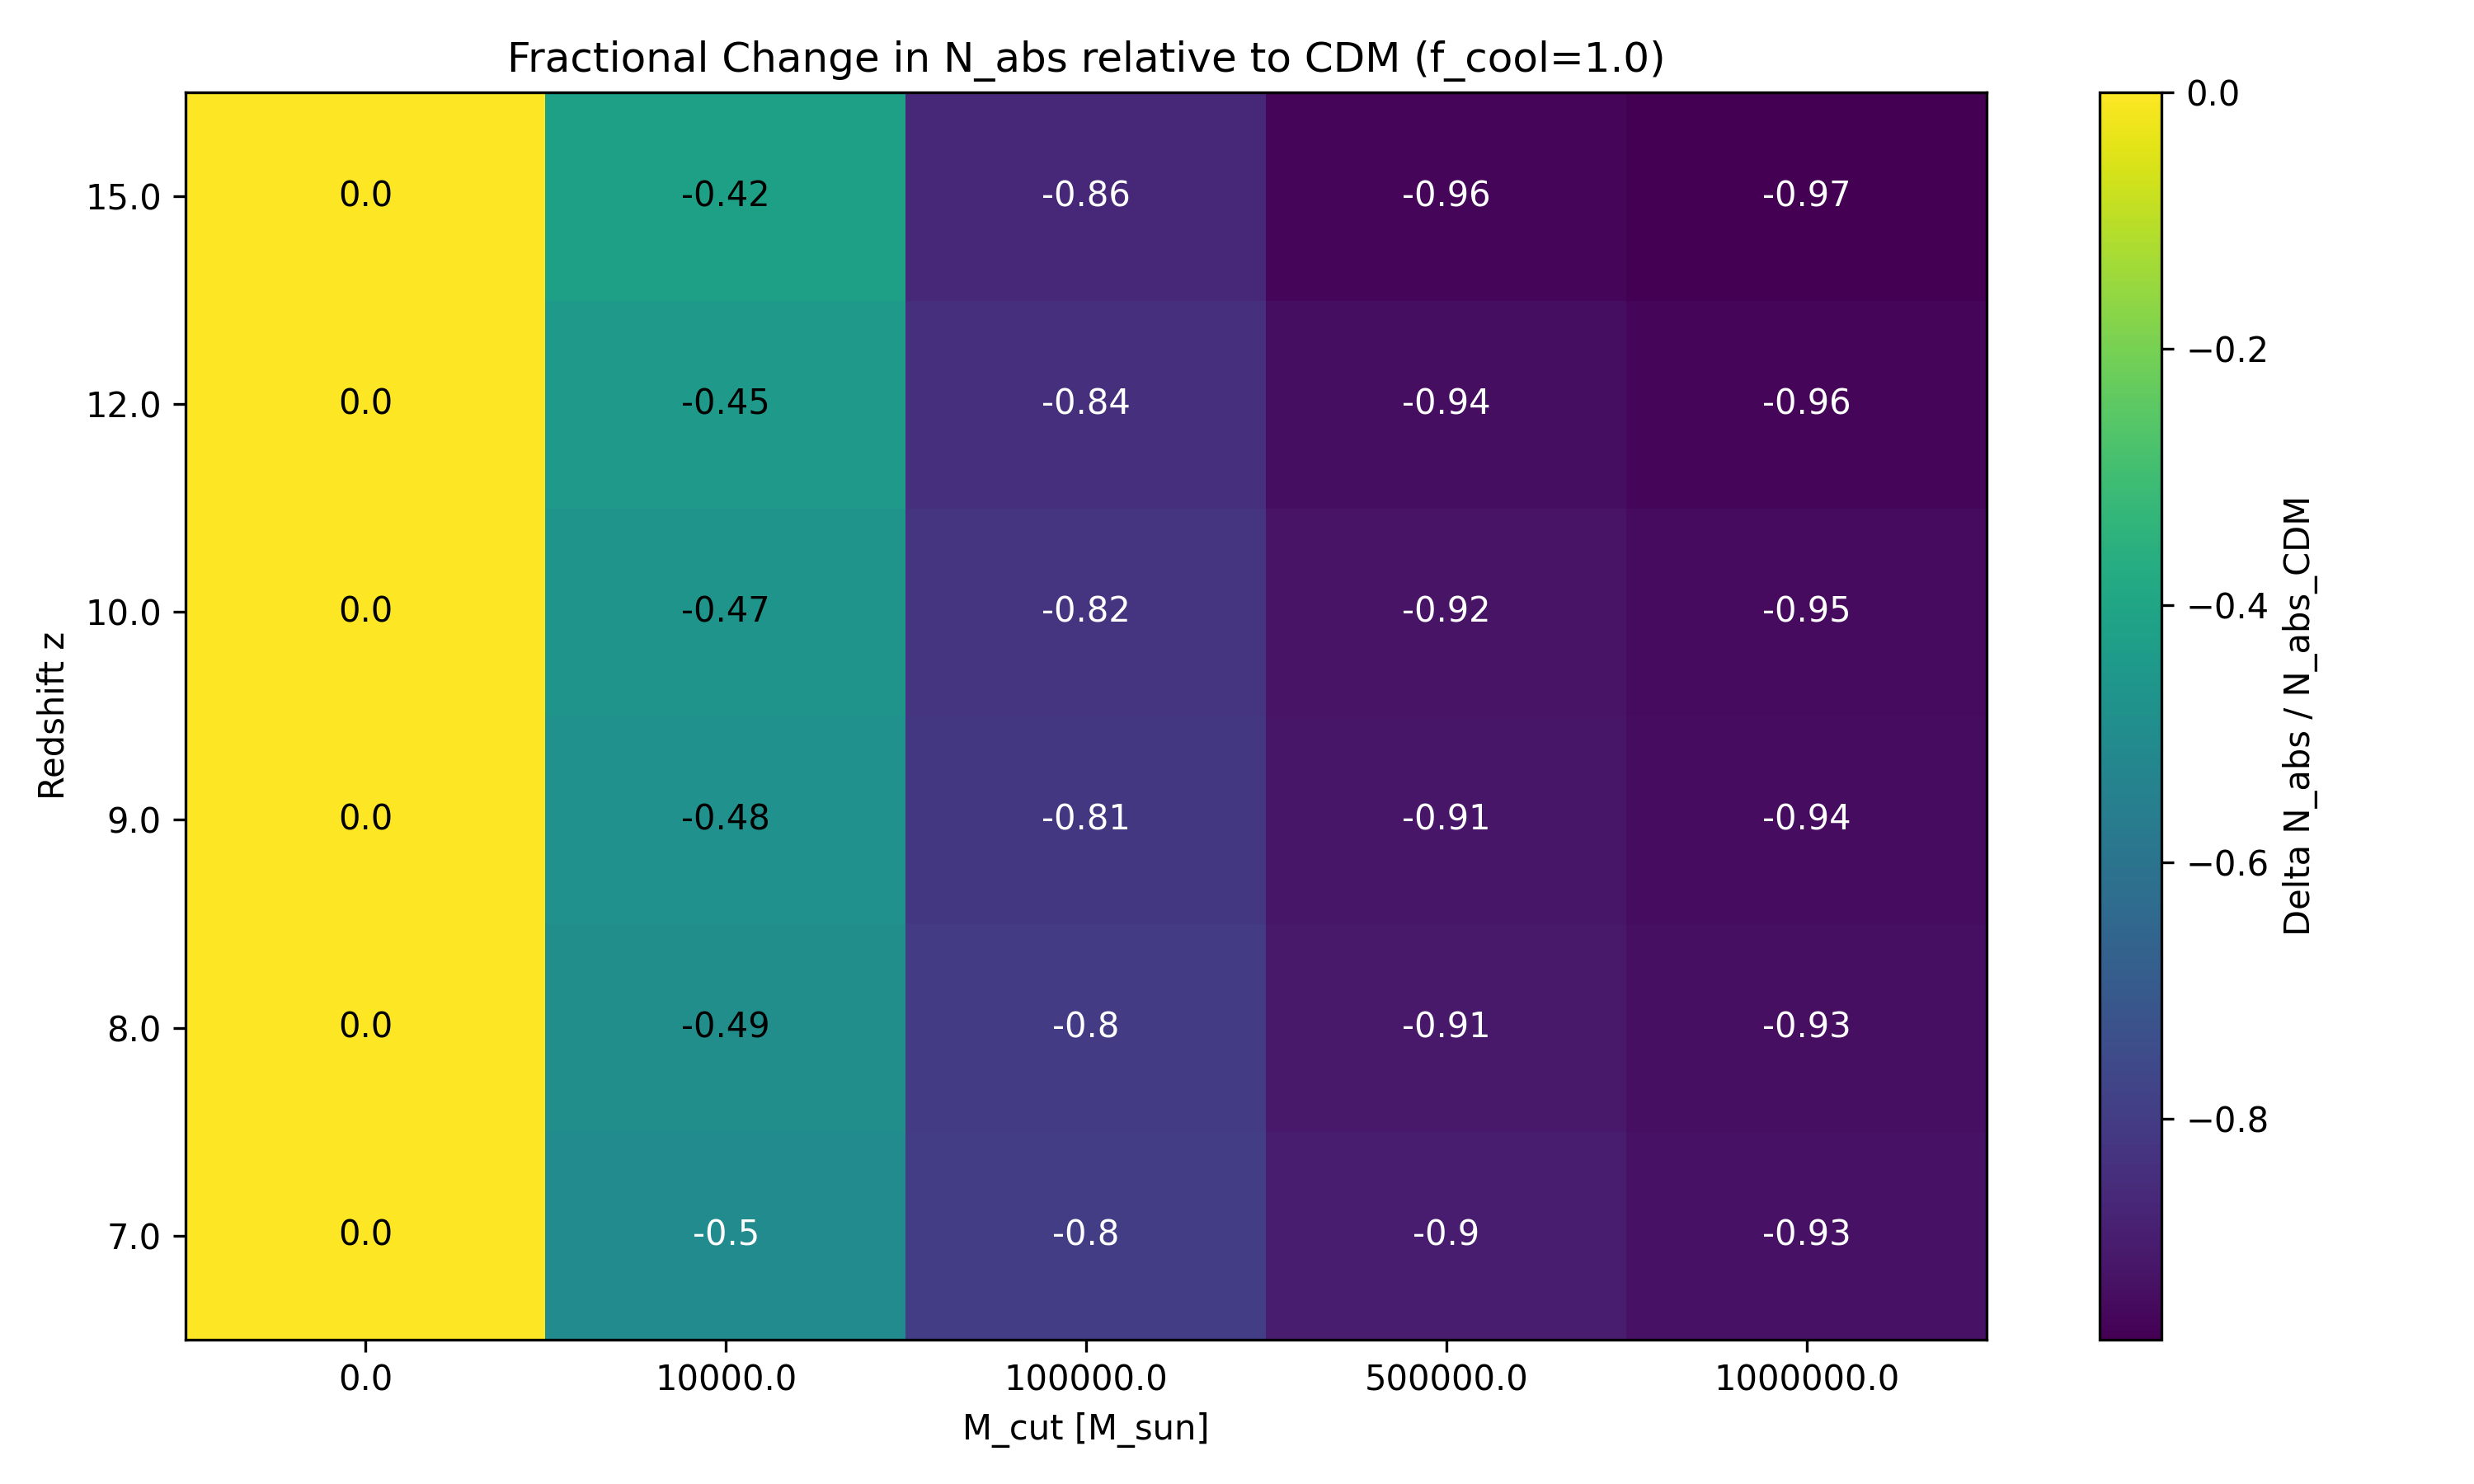
\includegraphics[width=0.5\textwidth]{../input_files/plots/step_2_frac_change_heatmap_3_20260413_122322.png}
    \caption{The fractional change in the total number of 21 cm absorbers ($N_{\text{abs}}$) relative to the standard CDM model, shown as a function of redshift $z$ and the structure suppression cutoff mass $M_{\text{cut}}$. The plot illustrates the profound impact of the kinematic suppression of small-scale structure caused by DM-baryon scattering. Even a modest cutoff mass of $M_{\text{cut}} = 10^4 \, M_\odot$ reduces the absorber count by approximately 40-50\%, while stronger interactions corresponding to $M_{\text{cut}} \ge 5 \times 10^5 \, M_\odot$ eliminate over 90\% of absorbers across all redshifts. This highlights the extreme sensitivity of the 21 cm forest observable to the structural effects of DM-baryon interactions.}
    \label{fig:image2}
\end{figure}

\subsection{A distinct fingerprint on the optical depth distribution}

Beyond simply reducing the total number of absorbers, structure suppression imprints a characteristic feature on the shape of the differential optical depth distribution, $dN/d\tau$. Since the lowest-mass minihalos typically produce absorption features with the lowest optical depths, a cutoff in the halo mass function preferentially removes these low-$\tau$ systems. The right panel of Figure \ref{fig:image0} illustrates this by showing the derivative $\partial N(>\tau) / \partial M_{\text{cut}}$, which confirms that the sensitivity to the cutoff mass is concentrated at the low optical depth end of the distribution. This change in shape provides a distinct "fingerprint" that can be used to distinguish the effects of dark matter scattering from astrophysical uncertainties, which typically rescale the overall amplitude of the distribution.

To quantify the statistical distinguishability of this fingerprint, we compute the Kullback-Leibler (KL) divergence, which measures the information gain when moving from a CDM model to one with a mass cutoff. As shown in Figure \ref{fig:image1}, two key trends emerge. First, for any given redshift, the KL divergence increases monotonically with $M_{\text{cut}}$, indicating that stronger interactions produce a more easily distinguishable signal. Second, for a fixed cutoff mass $M_{\text{cut}} \ge 10^5 \, M_\odot$, the KL divergence increases with redshift. This implies that the intrinsic physical signature of dark matter scattering on the shape of the $dN/d\tau$ distribution becomes more pronounced at earlier cosmic times, where the overall halo population is more heavily weighted towards the low-mass systems affected by the cutoff.

\begin{figure}[h!]
    \centering
    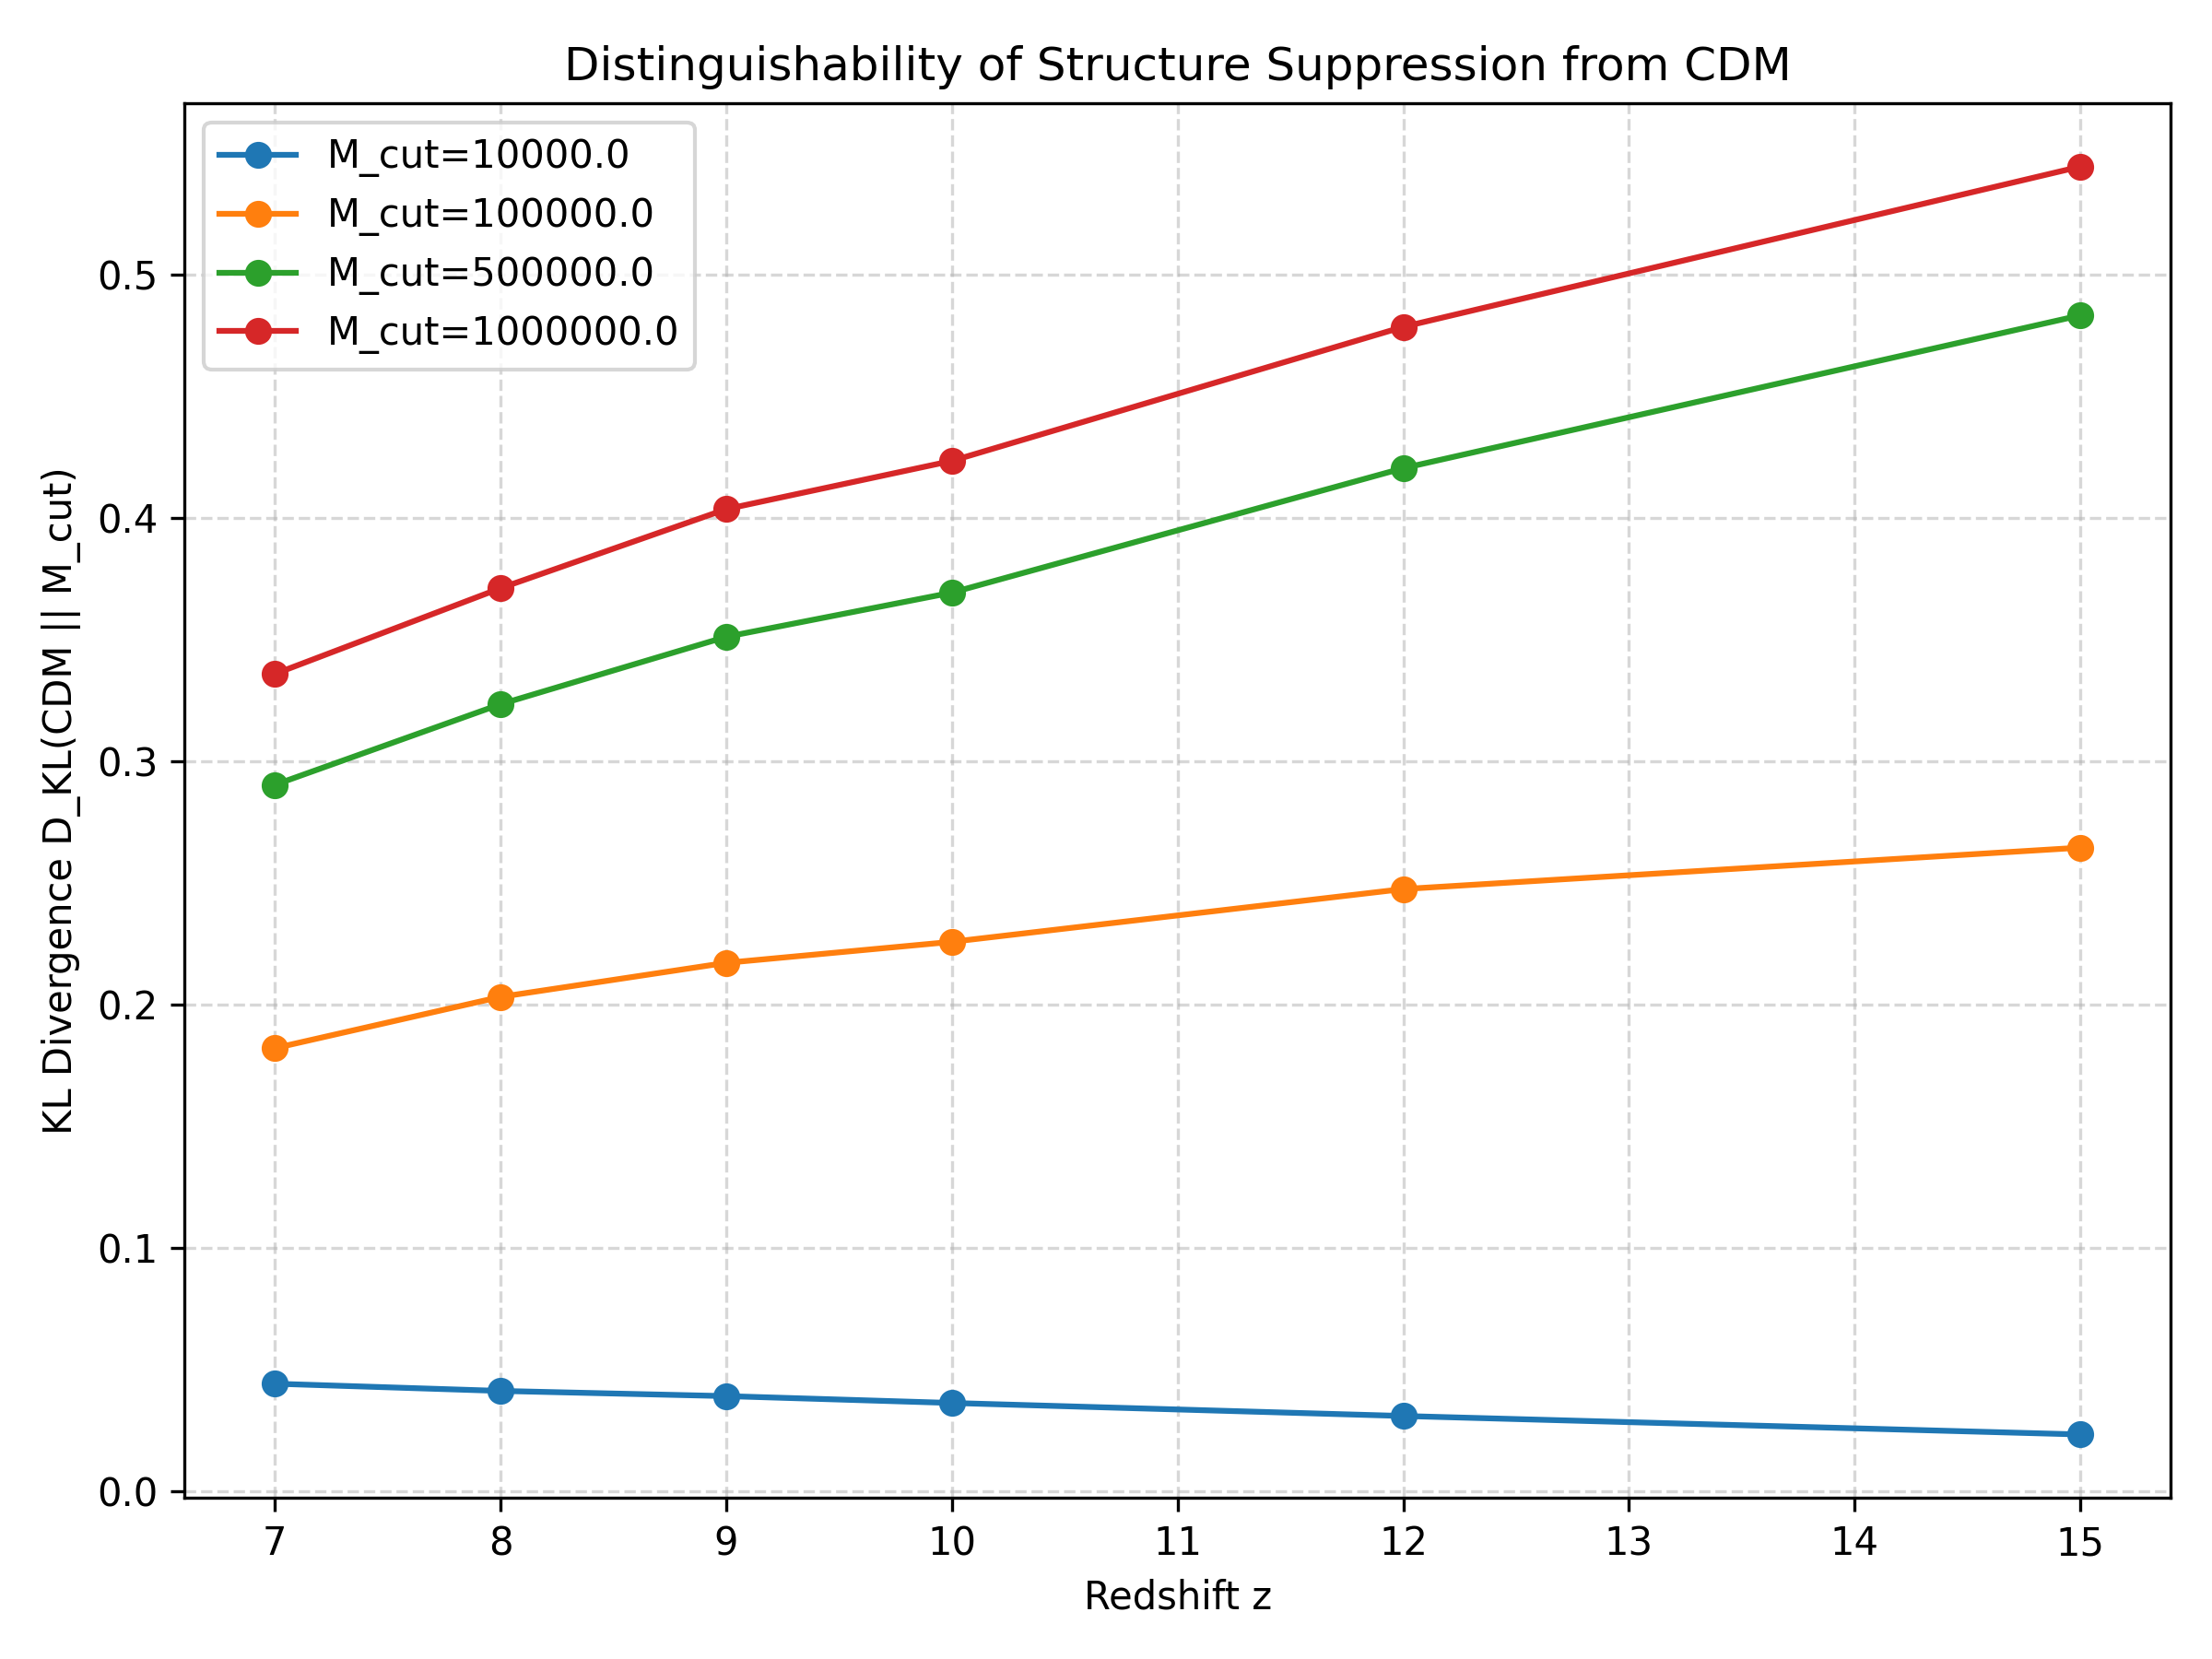
\includegraphics[width=0.5\textwidth]{../input_files/plots/step_2_KL_divergence_2_20260413_122322.png}
    \caption{The Kullback-Leibler (KL) divergence, $D_{\text{KL}}(\text{CDM} \parallel M_{\text{cut}})$, quantifying the statistical distinguishability between the differential optical depth distributions of a standard Cold Dark Matter (CDM) model and models featuring structure suppression due to DM-baryon scattering, parameterized by a cutoff mass $M_{\text{cut}}$. The divergence is plotted as a function of redshift for several values of $M_{\text{cut}}$. The plot demonstrates that distinguishability increases monotonically with the suppression scale ($M_{\text{cut}}$). For $M_{\text{cut}} \ge 10^5 \, M_\odot$, the divergence also grows with redshift, indicating that the observational fingerprint of structure suppression on the 21 cm forest becomes more pronounced at earlier cosmic times.}
    \label{fig:image1}
\end{figure}

\subsection{Fisher forecast and the optimal observational window}

While the intrinsic sensitivity to $M_{\text{cut}}$ is highest at early times, a realistic observational forecast must also account for the availability of background radio sources. We performed a Fisher matrix forecast for the parameter set \{$M_{\text{cut}}$, $f_{\text{cool}}$, $\bar{x}_{\text{HI}}$\}, incorporating a model where the number of available lines of sight, $N_{\text{los}}$, decreases at higher redshifts. This creates a fundamental trade-off: the physical signal is stronger at high redshift, but the statistical power to detect it is weaker due to increased Poisson noise.

Figure \ref{fig:image5} shows the result of this trade-off in the marginalized $1$-$\sigma$ uncertainty on the cutoff mass, $\sigma(M_{\text{cut}})$. The uncertainty is minimized at $z=7$ ($\sigma(M_{\text{cut}}) \approx 1127 \, M_\odot$), where the large number of sources provides the highest statistical power. However, the goal is not solely to minimize the uncertainty, but also to maximize the distinctness of the signal to separate it from astrophysical effects. For this reason, we identify an optimal observational window at $z \sim 8-10$. In this range, the statistical uncertainty remains low (e.g., $\sigma(M_{\text{cut}}) \approx 1907 \, M_\odot$ at $z=10$), while the intrinsic signature is significantly more distinct than at $z=7$, as quantified by the KL divergence (Figure \ref{fig:image1}). Furthermore, the off-diagonal elements of the Fisher matrix confirm that the shape-based fingerprint of $M_{\text{cut}}$ remains highly effective at breaking degeneracies with astrophysical parameters like the mean neutral fraction, $\bar{x}_{\text{HI}}$. This window therefore represents a strategic balance between signal strength and statistical precision.

\begin{figure}[h!]
    \centering
    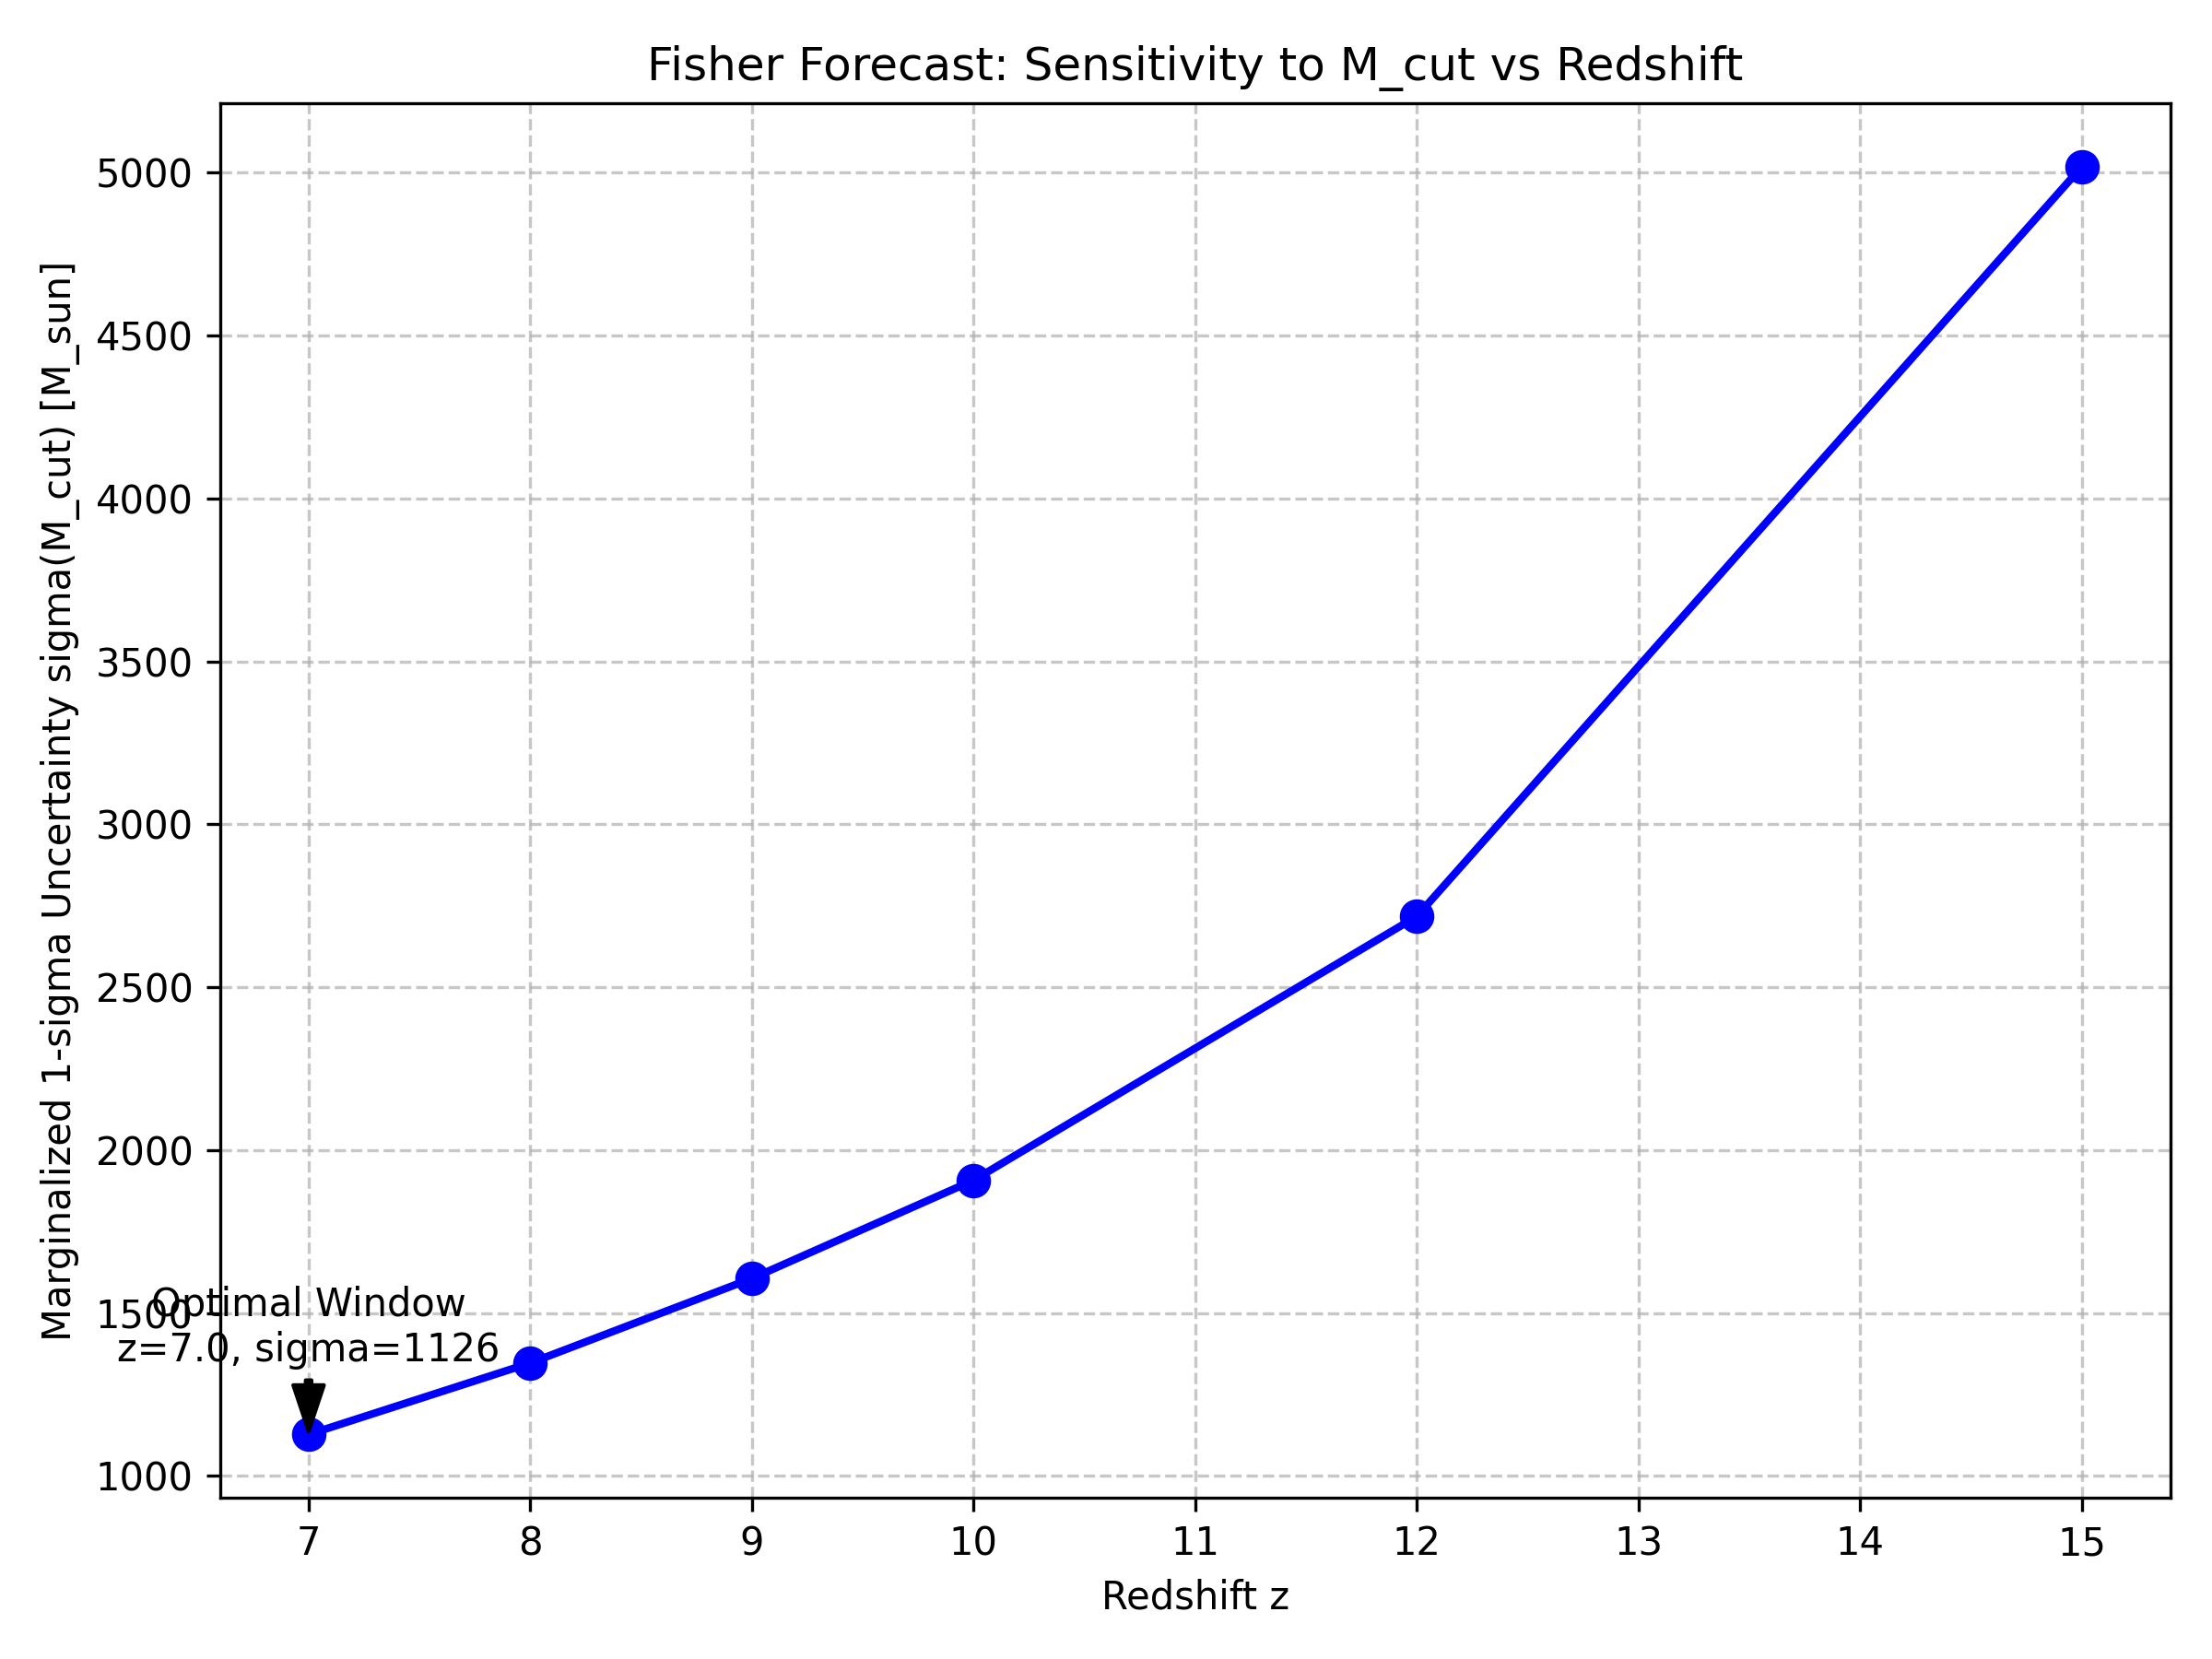
\includegraphics[width=0.5\textwidth]{../input_files/plots/step_4_fisher_sigma_Mcut_vs_z_1_20260413_122856.png}
    \caption{Fisher forecast for the marginalized 1-$\sigma$ uncertainty on the halo mass cutoff, $\sigma(M_{\text{cut}})$, as a function of redshift. The uncertainty increases monotonically with redshift, from $\sigma(M_{\text{cut}}) \approx 1127 \, M_\odot$ at $z=7$ to $\approx 5018 \, M_\odot$ at $z=15$. This trend is driven by the decreasing number of observable background radio sources at higher redshifts, which increases Poisson noise and dominates over the enhanced intrinsic physical sensitivity to structure suppression at earlier cosmic times.}
    \label{fig:image5}
\end{figure}

\subsection{Projected constraints on the dark matter-baryon cross-section}

The ultimate goal of this analysis is to translate the sensitivity to $M_{\text{cut}}$ into constraints on the fundamental dark matter-baryon scattering cross-section, $\sigma$. Figure \ref{fig:image3} shows the direct relationship between the number of absorbers and the cross-section normalization $\sigma_0/m_\chi$ at $z=10$ for both a velocity-independent ($n=0$) and a Coulomb-like ($n=-4$) interaction model. In both cases, an increasing cross-section leads to a monotonic decrease in the number of observable 21 cm absorbers.

Figure \ref{fig:image4} presents the projected sensitivity of the 21 cm forest across redshifts, showing the cross-section required to produce a 10\% or 20\% suppression in the total number of absorbers relative to the CDM prediction. The results indicate a transformative potential for constraining dark matter microphysics. For a velocity-independent ($n=0$) cross-section, a 10\% suppression measurement in the optimal window at $z=10$ would correspond to a sensitivity of $\sigma_0/m_\chi \approx 2.13 \times 10^{-26} \, \text{cm}^2/\text{GeV}$. For a Coulomb-like ($n=-4$) interaction, the sensitivity is even more extraordinary, reaching $\sigma_0/m_\chi \approx 2.13 \times 10^{-43} \, \text{cm}^2/\text{GeV}$. The extreme sensitivity to the $n=-4$ model arises from the $v^{-4}$ velocity dependence, which causes the interaction rate to become very large at the low relative velocities characteristic of the early universe.

These projected constraints are four to five orders of magnitude more stringent than current limits from the Cosmic Microwave Background. This highlights the unique power of the 21 cm forest, which leverages the suppression of small-scale structure to probe a region of dark matter parameter space inaccessible to other cosmological probes.

\begin{figure}[h!]
    \centering
    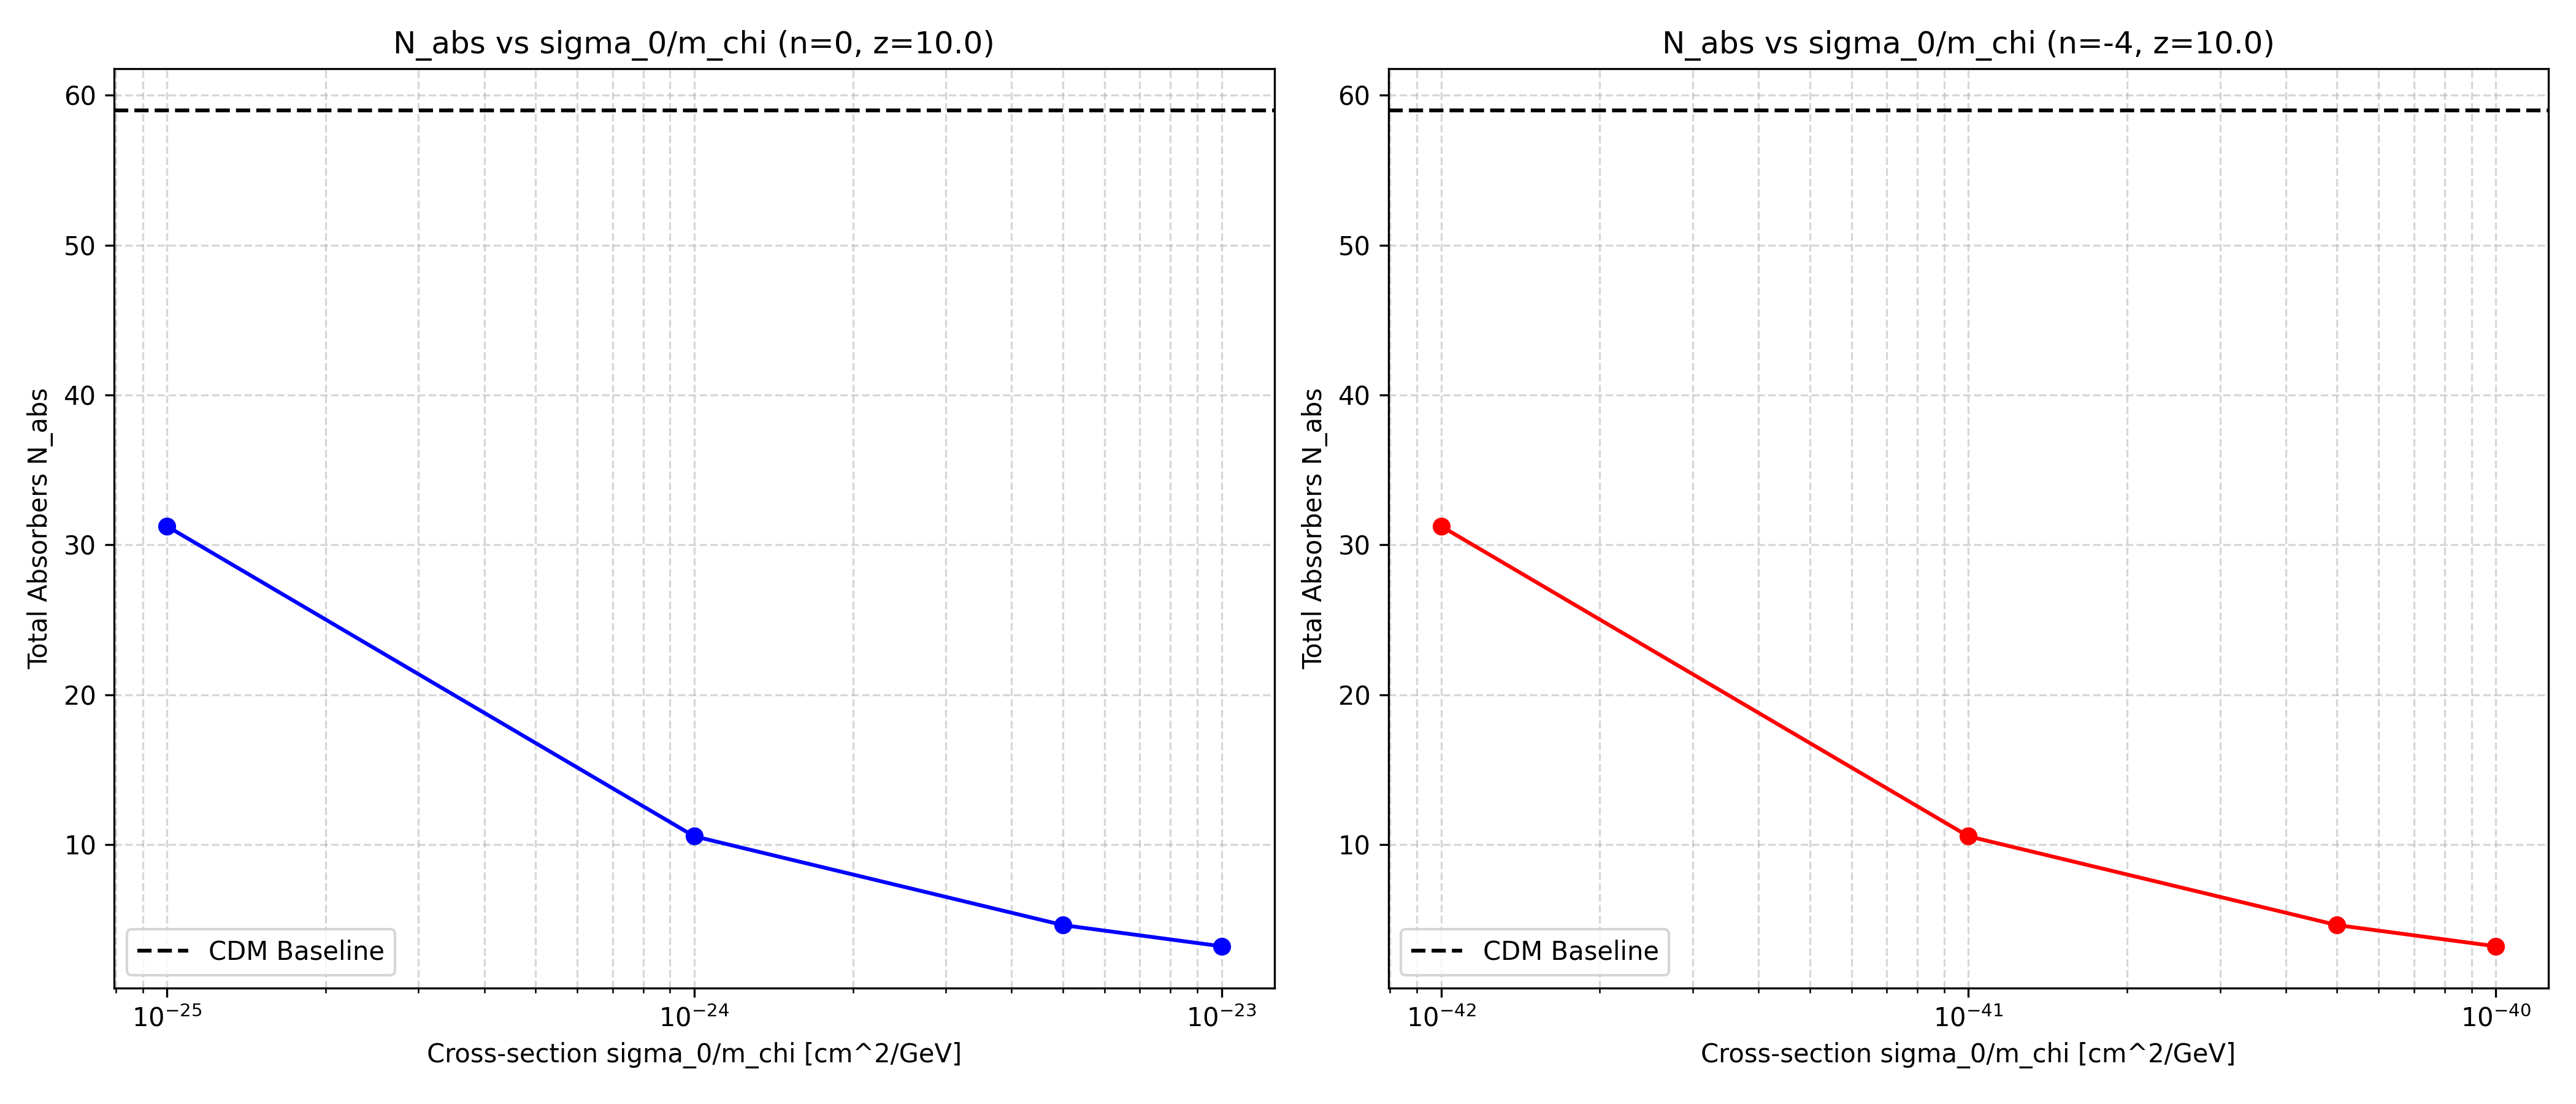
\includegraphics[width=0.5\textwidth]{../input_files/plots/step_3_Nabs_vs_sigma_20260413_122538.png}
    \caption{The total number of 21 cm forest absorbers, $N_{\text{abs}}$, at redshift $z=10$ as a function of the dark matter-baryon scattering cross-section, $\sigma_0/m_\chi$. The left panel corresponds to a velocity-independent interaction model ($n=0$), while the right panel shows a Coulomb-like model ($n=-4$). The plot demonstrates that increasing the interaction cross-section leads to a significant reduction in the number of absorbers compared to the standard Cold Dark Matter (CDM) baseline (dashed line), a direct consequence of the suppression of minihalo formation due to collisional damping.}
    \label{fig:image3}
\end{figure}

\begin{figure}[h!]
    \centering
    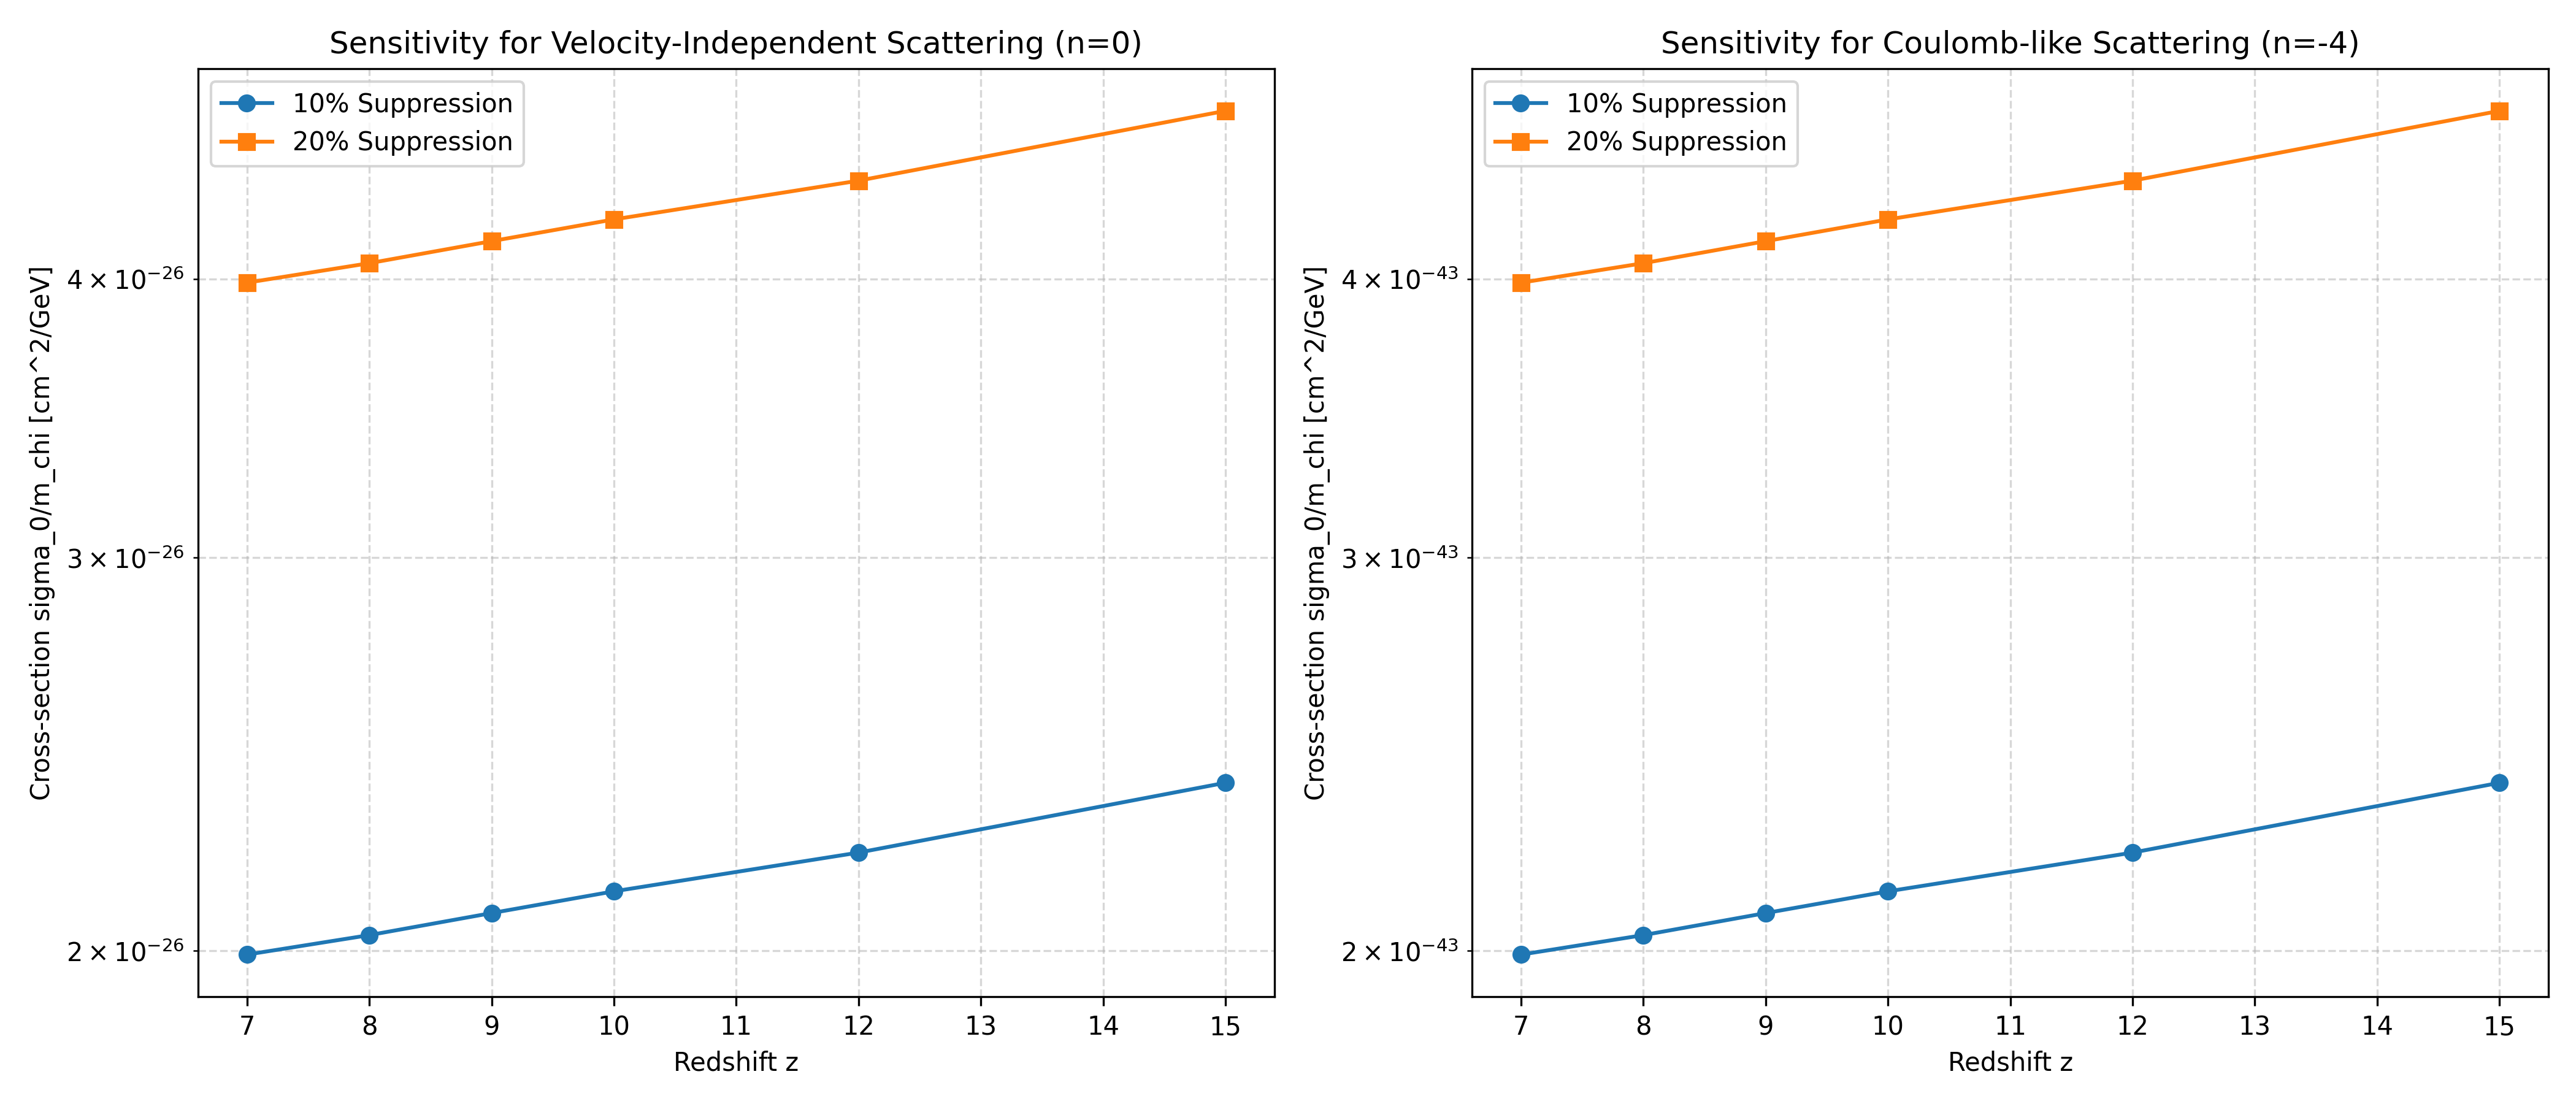
\includegraphics[width=0.5\textwidth]{../input_files/plots/step_3_sensitivity_curves_4_20260413_122634.png}
    \caption{Sensitivity of the 21 cm forest to the dark matter-baryon scattering cross-section ($\sigma_0/m_\chi$) as a function of redshift. The curves show the cross-section values required to suppress the total number of absorbers by 10\% (blue circles) and 20\% (orange squares) relative to the CDM prediction. Results are shown for a velocity-independent interaction ($n=0$, left panel) and a Coulomb-like interaction ($n=-4$, right panel). The probe is exceptionally sensitive to the Coulomb-like model, where the cross-section scales as $v^{-4}$, allowing constraints on $\sigma_0/m_\chi$ as low as $\sim 10^{-43} \, \text{cm}^2/\text{GeV}$.}
    \label{fig:image4}
\end{figure}

\section{Conclusions}
\label{sec:conclusions}
In this paper, we investigated the optimal strategy for detecting the signature of elastic scattering between dark matter and baryons using the 21 cm forest. Such an interaction suppresses the formation of small-scale structure, providing a powerful observational test of dark matter microphysics. Our goal was to identify the most sensitive observable, disentangle the dark matter signal from astrophysical effects, and determine the ideal redshift window for future observations.

To achieve this, we employed the \texttt{HAYASHI} semi-analytic framework to model the statistics of 21 cm absorbers from $z=7$ to $15$. We incorporated the effects of dark matter-baryon scattering through two channels: a cutoff in the halo mass function, $M_{cut}$, representing the suppression of structure formation, and a thermal cooling of the intergalactic medium. Using the differential optical depth distribution, $dN/d\tau$, as our primary observable, we performed a Fisher matrix forecast that included a realistic, redshift-dependent model for the number of background radio sources to project the constraining power of future radio observatories.

Our results demonstrate that the signature of dark matter-baryon scattering is overwhelmingly dominated by the kinematic suppression of low-mass minihalos. The thermal cooling channel was found to have a negligible impact on the 21 cm absorption statistics, as the signal is already saturated in the cold, high-redshift intergalactic medium. The suppression of minihalos imprints a distinct fingerprint on the shape of the optical depth distribution, preferentially removing low-$\tau$ absorbers. This shape-based signature provides a powerful discriminant to distinguish the dark matter interaction from astrophysical uncertainties that tend to rescale the overall amplitude of the signal.

We learned that there is a fundamental trade-off between intrinsic physical sensitivity and statistical constraining power. While the signature of structure suppression becomes more pronounced at higher redshifts, the decreasing number of bright background radio sources weakens the statistical power of the measurement. Our Fisher analysis synthesized these competing effects, identifying an optimal observational window at $z \sim 8-10$. This window represents a strategic balance, maximizing the distinguishability of the signal while retaining sufficient statistical power for a robust detection.

In conclusion, the 21 cm forest is a uniquely powerful probe of the fundamental nature of dark matter. By targeting the characteristic suppression of low optical depth systems within the optimal redshift window of $z \sim 8-10$, future radio observatories can place constraints on the velocity-independent dark matter-baryon scattering cross-section that are four to five orders of magnitude more stringent than current limits from the Cosmic Microwave Background. This work establishes a clear observational pathway for leveraging the 21 cm forest to explore a vast and otherwise inaccessible region of the dark matter parameter space.


\bibliography{bibliography_valency}{}
\bibliographystyle{unsrt}

\end{document}
